\documentclass[convert]{standalone}

\usepackage{tikz}
\pagestyle{empty}

% INT_AY22_L03_Fig11_vy_v_time_graph.png

\begin{document}
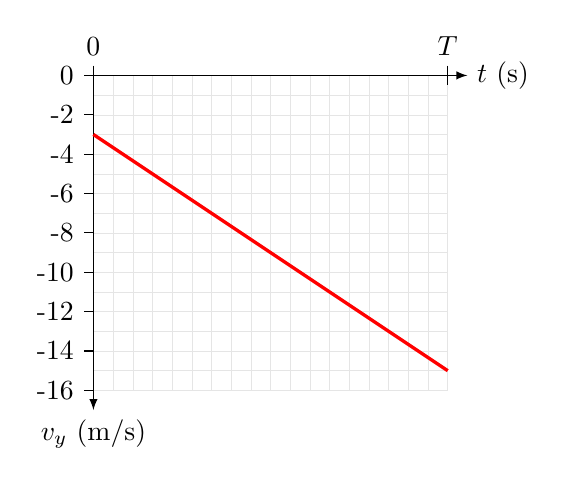
\begin{tikzpicture}[> = latex]

	% Axes + grid
	
	\draw [very thin, gray!20, step = 0.25 cm] (0, 0) grid (4.5, 4);
	
	\draw [<->] (0, -0.25)  node [below] {$v_y$ (m/s)} -- (0, 4) -- (4.75, 4) node [right] {$t$ (s)};

	% Axis labels
	
	\draw (0, 4.125) node [above] {$0$} -- (0, 3.875);
	\draw (4.5, 4.125) node [above] {$T$} -- (4.5, 3.875);
	
	\foreach \y in {0, -2, ..., -16}
		\draw (0, {0.25 * \y + 4}) -- (-0.125, {0.25 * \y + 4}) node [left] {\y};
		
	% Curve
	
	\draw [very thick, red] (0, 3.25) -- (4.5, 0.25);

\end{tikzpicture}
\end{document}